En esta sección, vamos a comprobar empíricamente que nuestro algoritmo tiene una complejidad temporal de $O(n^3)$.

En este primer caso utilizamos instancia aleatorias variando el tamaño de n. A su vez, utilizamos distintos tamaños de k.

\begin{figure}[H]
  \begin{minipage}{0.5\linewidth}
    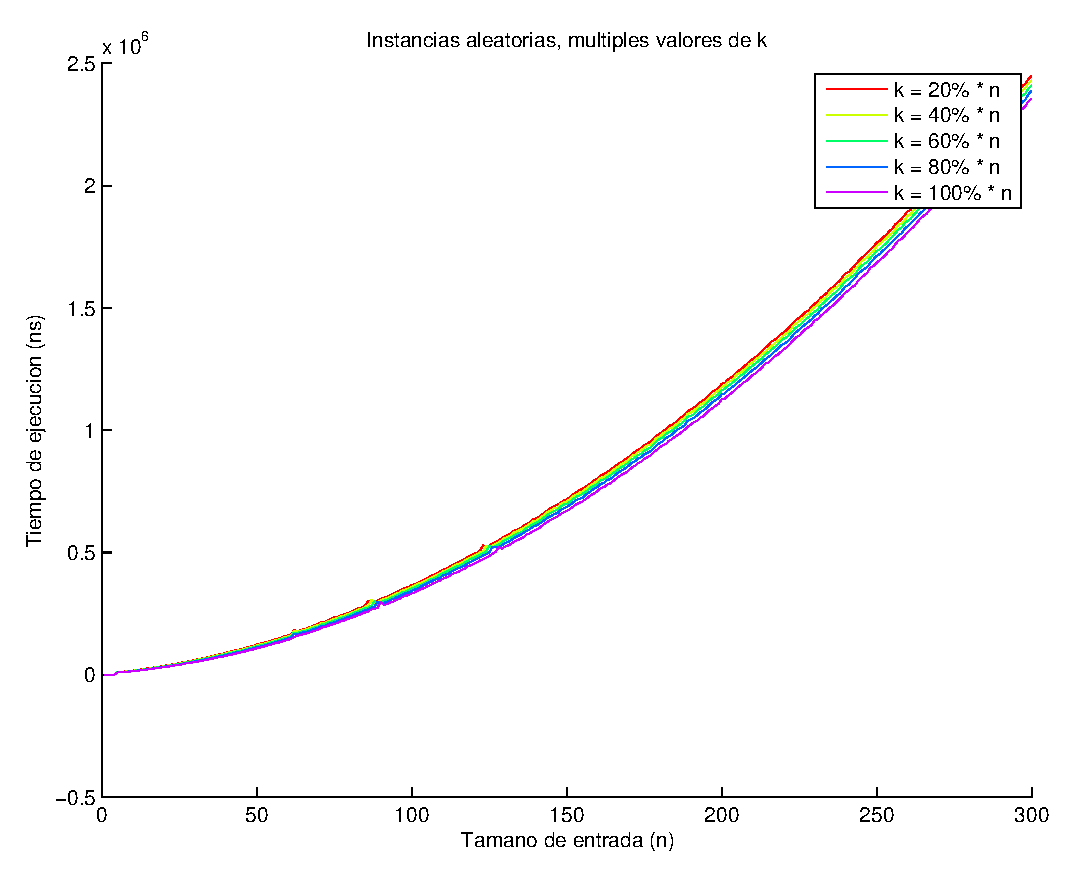
\includegraphics[width=\linewidth]{img/problema2/instancia_aleatoria_varios_k.eps}
    \caption{Tiempo de ejecución instancia aleatoria}\label{fig:problema2-k}
  \end{minipage}
  \hfill
  \begin{minipage}{0.5\linewidth}
    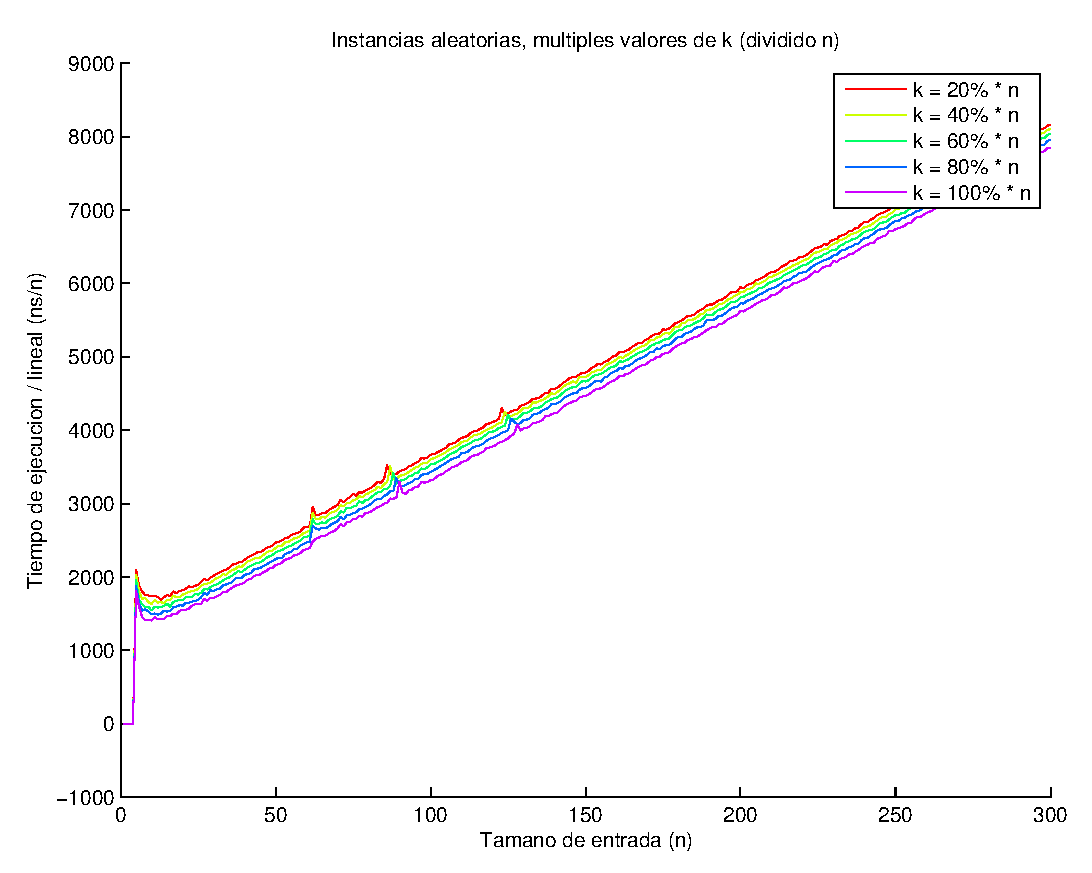
\includegraphics[width=\linewidth]{img/problema2/instancia_aleatoria_varios_k_div_n.eps}
    \caption{Idem, dividido por $n^2$}\label{fig:problema2-k-n}
  \end{minipage}
\end{figure}

En la figura \ref{fig:problema2-k} no podemos notar la complejidad temporal de la función. Por esto, dividimos por $n$ y plasmamos ese resultado en la figura \ref{fig:problema2-k-n}. En esta última figura, vemos claramente que $T(n) / n$ es una recta. De esta manera, pudimos comprobar empíricamente que $T(n)$ tiene una complejidad temporal de $O(n^2)$, lo cual demostramos anteriormente.